\documentclass[10pt]{seminar} 

\renewcommand{\baselinestretch}{1}

\usepackage{amsmath}

\renewcommand{\printlandscape}{\special{landscape}}

\usepackage{ulem}



\input{seminar.bug}

%\usepackage{fancybox}

\usepackage{epsfig}

%\usepackage{times}


\usepackage{amssymb}

\usepackage{amscd}

\usepackage{graphics}

\usepackage{pstricks}

%\usepackage{chicago}

%\usepackage{fullpage}

\slideframe{none}

\begin{document}

\newtheorem{proposition}{Proposition}

\newtheorem{definition}{Definition}

\newtheorem{corollary}{Corollary}

\newtheorem{theorem}{Theorem}

\newtheorem{lemma}{Lemma}

\def\argmax{\mathop{\rm argmax}\limits}  


%\slideframe{Oval}

\sffamily 


\begin{slide}
\begin{center}

 Sequences, Series, Limits \& Continuity
 \end{center}
 
 \newslide

A \textit{sequence} of real numbers is a function, $u$, mapping $\mathbb{N}$ to $\mathbb{R}$

\begin{itemize}
\item We will be dealing with infinite sequences
\item Written $u(1), u(2), u(3), ... $, or $(u_1, u_2, u_3, ...)$
\item The sequence is written $\{u_n\}$
\item Example of a sequence $$u_n={{3n^2}\over{n^3+9}}$$ which gives the sequence  $${3\over 10},{12\over 17}, {48\over 73}, ...$$
\end{itemize}


\newslide
Arithmetic sequences

\begin{itemize}
\item An arithmetic sequence is a sequence $\{u_n\}$ in which $$u_{n+1}-u_n$$ is constant for all $n$
\item Equivalent to saying that for some numbers $a, d$, the sequence looks like $$a, a+d, a+2d, a+3d, ...$$ or $$u_n=a+(n-1)d$$
\item Is this sequence arithmetic? (If so, what are $a, d$?) $$u_n=14-5n$$ %a=9, d=-5!

\item Is this one? $$u_n=5^{-n}$$

\end{itemize}

\newslide

Arithmetic sequences: Each term is obtained by adding same number to previous term

\ \\Geometric sequences: Each term is obtained by multiplying previous term by same number

\begin{itemize}
\item Equivalent to saying that for some numbers $a, x$ the sequence looks like $$a, ax, ax^2, ax^3, ...$$ or $$u_n=ax^{n-1}$$

\item What are $a, x$ for this geometric sequence? $$u_n=5^{-n}$$ %a=1/5, x=1/5
\end{itemize}

\newslide
Limits of sequences

\begin{itemize}
\item The \textit{limit} of a sequence describes what happens to $u_n$ as $n$ becomes large

\item A sequence $\{u_n\}$ tends to the limit $z$ if for \textit{any} positive real number $\epsilon$ there is a positive integer, $N$, such that:

$$|u_n-z|<\epsilon \hbox{ for all }n>N.$$

\item Also written as  $$\lim u_n=z$$ $$\lim_{n\rightarrow \infty}u_n=z$$ $$u_n\rightarrow z \hbox{ as } n\rightarrow \infty$$

\end{itemize}

\newslide An example: Let's show that $u_n={1\over n}$ tends to limit $z=0$

Convergent sequence:  $\lim u_n=z$ if for \textit{any}  $\epsilon>0$ there is a positive integer, $N$ such that $|u_n-z|<\epsilon \hbox{ for all }n>N.$

\ \\Put differently, for any $\epsilon>0$, \textbf{IF} $n>N$ \textbf{THEN} $|u_n-z|<\epsilon$.

\ \\Take any $\epsilon>0$ (it can be arbitrarily small).  Let $N $ be any integer greater than ${1\over \epsilon}$.  Note that $N>{1\over \epsilon}$ implies that $\epsilon>{1\over N}$.

\ \\ Then for all $n>N$, we have $$|u_n-0|={1\over n}<{1\over N}<\epsilon.$$

\ \\It follows that our sequence $u_n={1\over n}$ tends to the limit $z=0$.

\newslide
Definitions:

\ \\A sequence that tends to a limit is called \textit{convergent}; a sequence that doesn't is called \textit{divergent}

\ \\A sequence that tends to infinity (or negative infinity) is divergent, but a sequence doesn't have to tend to infinity to be divergent (what's an example of a divergent sequence that doesn't tend to infinity?)

\ \\A \textit{Cauchy } sequence of real numbers is a sequence whose elements cluster around some number as $n$ gets large.  Since we are dealing with the real numbers, a Cauchy sequence is equivalent to a convergent sequence. %Rationals a good example of a metric space that is not complete; Convergence implies Cauchy but not vice versa since a Cauchy sequence can limit to an irrational number; useful when you want to show convergence without using the limit point

$$\{x_n\} \hbox{ is Cauchy if } \forall\epsilon>0, \exists N\in \mathbb{N}:|x_m-x_n|<\epsilon \hbox{ when }m, n>N$$

\newslide

$$\{x_n\} \hbox{ is Cauchy if } \forall\epsilon>0, \exists N\in \mathbb{N}:|x_m-x_n|<\epsilon \hbox{ when }m, n>N$$

We can show the sequence defined by $x_n=n$ is not convergent:

\ \\$|x_n-x_m|=|n-m|\geq 1$ for all $n, m$.  Thus, for $\epsilon=1$ there is no $N$ such that $|x_n-x_m|<\epsilon$ whenever $n, m>N$.  Therefore $\{x_n\}$ is not Cauchy, and does not tend to a limit.

\newslide
Working with limits

\ \\Fact 1: For a real number $x$, $\lim_{n\rightarrow\infty}x^n=0$ if and only if $-1<x<1$.

\ \\Fact 2: For a real number $b$, $\lim_{n\rightarrow\infty}n^b=0$ if and only if $b<0$.

\ \\ As $n\rightarrow \infty$, what's the limit of $$u_n={{n+1}\over{2n}} $$ %1/2

\newslide Claim: If $\lim u_n=z$ then $\lim |u_n |=|z|$

\ \\Proof: If $\lim u_n=z$ then for any $\epsilon>0$,  $|u_n-z|<\epsilon$ for $n$ large.  First, note that for real numbers $a, b$ we have $$||a|-|b||\leq |a-b|$$ (the ``reverse triangle inequality").  This basically proves our result: For any $\epsilon >0$ we have $|u_n-z|<\epsilon$ for $n$ large, and consequently $||u_n|-|z||<|u_n-z|<\epsilon$.  Thus, $\lim |u_n |=|z|$. $\Box$

\ \\Does the converse hold? (If $\lim |u_n |=|z|$  then $\lim u_n=z$) %Nope, $x_n=(-1)^n$

%Reverse triangle: |x|+|y-x|>|x+y-x|=|y| and |y|+|x-y|>|y+x-y|=|x|
%So |y-x|>|y|-|x| and |x-y|>|x|-|y|

\newslide

What is the limit of 

$$u_n={{(-1)^n(n+1)^2}\over{n^4}}?$$ %0

\ \\Hint: We can start by expanding the numerator.

\ \\What would happen if we replaced $(n+1)^2$ with $(n+1)^4$?  \\Don't do whole calculation!

\newslide

Series

\begin{itemize}
\item The series defined by a sequence $\{u_n\}$ is the sequence $\{s_n\}$ with $$s_1=u_1, s_2=u_1+u_2, s_3=u_1+u_2+u_3, ...$$ and more generally $$s_n=\sum_{r=1}^{n}u_r$$
\end{itemize}

\newslide
Summing algebraic sequences

\ \\First, the natural numbers $$s_n=1+ 2+ ...+(n-1)+  n$$
 $$s_n=n + (n-1) + ...+ 2+ 1$$
 
 Adding these together we get 
 
 $$2s_n=(1+n)+(1+n)+...+(1+n)= n(1+n)$$
 
 The first $n$ terms of the natural numbers sum to 
 $$s_n={1\over 2}n(1+n)$$

\newslide

Recall that a general arithmetic sequence is $u_n=a+(n-1)d$

\ \\We can use the same trick to find the sum of the first $n$ terms of the sequence:

$$u_n=a+(a+d)+(a+2d)+...+(a+(n-2)d)+(a+(n-1)d)$$
$$u_n=(a+(n-1)d)+(a+(n-2)d)+...+(a+2d)+(a+d)+a$$
$$2u_n=n\left(2a+(n-1)d\right)$$
$$u_n=an+n\left({{(n-1)d}\over{2}}\right)$$

\newslide
Summing geometric sequences: $s_n=a+ax+ax^2+...+ax^{n-1}$

\ \\Multiplying by $x$ we get 
$$xs_n=ax+ax^2+...+ax^n$$
Let $$t=ax+ax^2+...+ax^{n-1}$$ Then $s_n=a+t$ and $xs_n=t+ax^n$   $$s_n-xs_n=a-ax^n$$ so 
$$s_n(1-x)=a-ax^n,$$ and finally $$s_n=a\left({{1-x^n}\over{1-x}}\right)$$

\newslide
Convergence of geometric series

\ \\We will often care about the limit of a series as $n\rightarrow \infty$

\ \\For a geometric series, $$s_n=a\left({{1-x^n}\over{1-x}}\right)$$

\ \\We know that $x^n\rightarrow 0$ as $n\rightarrow\infty$ if and only if $|x|<1$

\ \\If $|x|<1$ then $\lim_{n\rightarrow\infty}s_n=a\left({{1-0}\over{1-x}}\right) = {a\over{1-x}}$

\newslide
Divergence of geometric series

\ \\Fact (\textit{term test} for any series): If $\lim_{n\rightarrow \infty} k_n\not=0$ then $\sum_{n=1}^\infty k_n$ diverges

\ \\For a geometric series, $k_n=ax^{n-1}$

\ \\We know that $x^n\rightarrow 0$ as $n\rightarrow\infty$ \underline{if and only if} $|x|<1$

\ \\Therefore, a geometric series diverges whenever $|x|\geq 1$
\newslide

Ex: Sequences in the social sciences (\textit{exponential discounting})

\ \\Suppose that I plan to consume $x$ units of cake in each of an infinite number of time periods, $t=1, 2, 3, ...$

\ \\I discount the utility I'll receive from future consumption by a term $0<\delta<1$, so that I value today's consumption fully as $u(x)$, tomorrow's as  $\delta u(x)$, the day after's as $\delta^2 u(x)$...

\ \\My expected utility over time is $$\sum_{t=0}^\infty \delta^t u(x) = {{u(x)}\over{1-\delta}}$$

\ \\``Cake eating problem": How to allocate a fixed unit of x over this infinite stream \textit{today} in order to maximize my lifetime utility

\newslide
Limits and continuity

\ \\Let $f(x)=y$ be a real-valued function, where the domain of $f$ is either all the real numbers or some interval of real numbers 

\ \\The \textit{domain} of $f:X\rightarrow Y$ is $X$, the ``input" values of $f$; \\$Y$ is the \textit{codomain}  

\ \\The \textit{range} of $f$ (or \textit{image}) is the set of values of $Y$ that $f$ actually takes


\newslide

\begin{center}$f(x)$ ``tends to the limit $l$ as $x$ approaches $x_o$" \end{center}

 $$f(x)\rightarrow l \hbox{ as }x\rightarrow x_o$$
 
 $$\lim_{x\rightarrow x_o}f(x)=l$$

These statements mean that $f(x)$ can attain values as close as we want to $l$ for all $x$ sufficiently close (but not equal) to $x_o$

\newslide

More formally:  $$f(x)\rightarrow l \hbox{ as }x\rightarrow x_o$$ if for any $\epsilon>0$ we can choose a $\delta>0$ such that $$|f(x)-l|<\epsilon \hbox{ for all }x \hbox{ such that }0<|x-x_o|<\delta$$

\ \\Example: $f(x)=20-10x$.  Then $\lim_{x\rightarrow 1} f(x)=10$.  To prove this using $(\delta, \epsilon)$ we want to show that for \textit{any} $\epsilon>0$ we can find a $\delta>0$  so that

$$|f(x)-10|<\epsilon \hbox{ whenever }|x-1|<\delta$$

\newslide

$$|f(x)-10|<\epsilon \hbox{ whenever }|x-1|<\delta$$

$$|(20-10x)-10|<\epsilon \hbox{ whenever } |x-1|<\delta $$

$$|10-10x|<\epsilon \hbox{ whenever } |x-1|<\delta $$

$$10 |x-1|<\epsilon \hbox{ whenever } |x-1|<{\epsilon\over 10 }$$

For any $\epsilon$ we could choose, this holds for $\delta={\epsilon\over 10}$ \\(Plug in some examples: try $\epsilon=5$)

\newslide
$f(x)=20-10x$

\ \\ $\lim_{x\rightarrow 1} f(x)=10$

\vspace{.1in}
\begin{center}
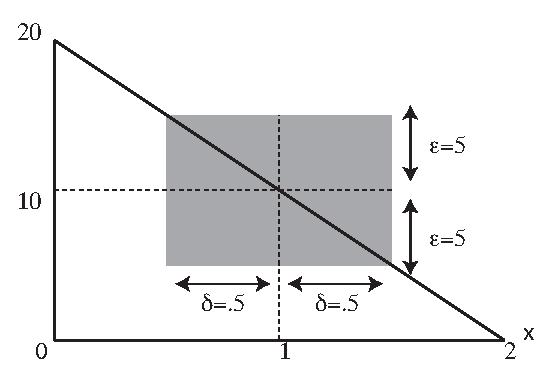
\epsfig{file=deltaE.eps, scale=.75}
\end{center}

\newslide
Important points:

\ \\$\lim_{x\rightarrow x_o}f(x)$ might or might not equal $f(x_o)$

\begin{itemize}
\item It could be \textit{different than} $f(x_o)$

 \[
    f(x)=\left\{
                \begin{array}{lll}
                  +1&\hbox{if } x\not=4\\
                  -1&\hbox{if } x=4
                \end{array}
              \right.
  \]

%$\lim\limits_{x\rightarrow 4}f(x)=1$ while $f(4)=-1$

\item It could be \textit{undefined}

 \[
    f(x)=\left\{
                \begin{array}{lll}
                  +1&\hbox{if } x<0\\
                  -1&\hbox{if } x\geq 0
                \end{array}
              \right.
  \]

\end{itemize}


\newslide
Operations with limits

\ \\Suppose that $f(x)\rightarrow l$ and $g(x)\rightarrow m$ as $x\rightarrow x_o$.  Then:

\begin{enumerate}
\item $\lim_{x\rightarrow x_o} f(x)+g(x)=l+m$
\item $\lim_{x\rightarrow x_o}f(x)g(x)=lm$
\item $\lim_{x\rightarrow x_o}{{f(x)}\over{g(x)}}={l\over m}$ if $m\not=0$

\begin{itemize}
\item For this last case, if $m, l=0$ or $m, l=\infty$ we have an \textit{indeterminate form}, and the limit of ${{f(x)}\over{g(x)}}$ might or might not exist. We use L'H\^opital's Rule in this case (requires calculus so we'll hold off on this). 
\end{itemize}
\end{enumerate}

\newslide

One-sided limits

\ \\$f(x)$ tends to $l$ as $x$ approaches $x_o$ from above (below): $\lim_{x\downarrow x_o}f(x)=l$

 \[
    f(x)=\left\{
                \begin{array}{lll}
                  +1&\hbox{if } x<0\\
                  -1&\hbox{if } x\geq 0
                \end{array}
              \right.
  \]
  
  
  
In this case, $\lim_{x\downarrow 0}f(x)=-1$ and $\lim_{x\uparrow 0}f(x)=1$
  
  \begin{center}
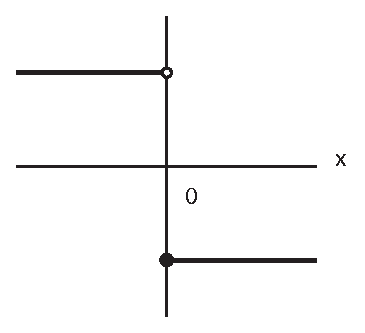
\epsfig{file=limitAbove.eps, scale=.5}
\end{center}


\newslide
Continuity

\begin{itemize}
\item If $\lim_{x\rightarrow x_o}f(x)=f(x_o)$ we say that $f$ is \textit{continuous} at $x_o$; \\if not, the function is \textit{discontinuous} at $x_o$
\item If a function $f$ is continuous for every $x$ then $f$ is a \textit{continuous function}
\item Most important thing about continuous functions: $f$ is continuous if arbitrarily small changes in $x$ produce arbitrarily small changes in $f(x)$. These changes can be as small as we want them to be.

\item In other words, we can make the change in $f(x) $ as small as we like if we make the change in $x$ small enough.


\end{itemize}

\newslide

Continuity: Small changes in $x$ map into small changes in $f(x)$


\ \\ A function $f: \mathbb{R}\rightarrow \mathbb{R}$ is continuous at point $x_o\in \mathbb{R}$ if for any $\epsilon>0$ there exists a $\delta>0$ such that $$\text{ If } |x_o-x|<\delta \text{ then} |f(x_o)-f(x)|<\epsilon$$



\newslide
The intermediate value theorem

\ \\If the function $f(x)=y$ is continuous for all $a\leq x\leq b$ then $f$ takes every value between $f(a)$ and $f(b)$

\begin{center}
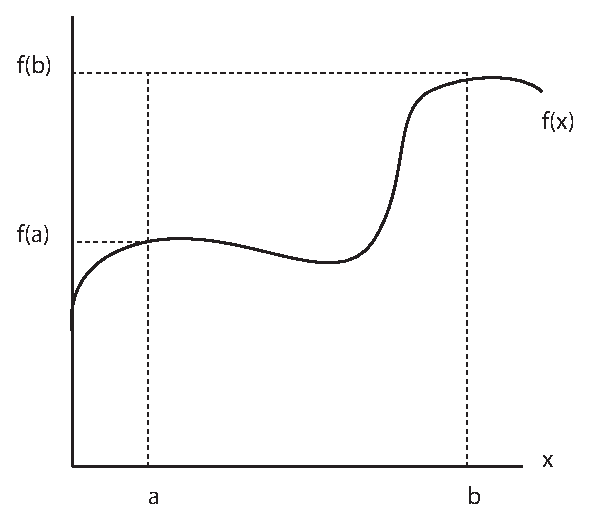
\epsfig{file=intVal.eps, scale=.6}

\end{center}
\end{slide}
\end{document}








